% AMO2 HW2

\subsection{Problem 2}
\subsubsection{(a)}

Plots of $V_{ij}(R)$
\begin{figure}[ht]
\centering
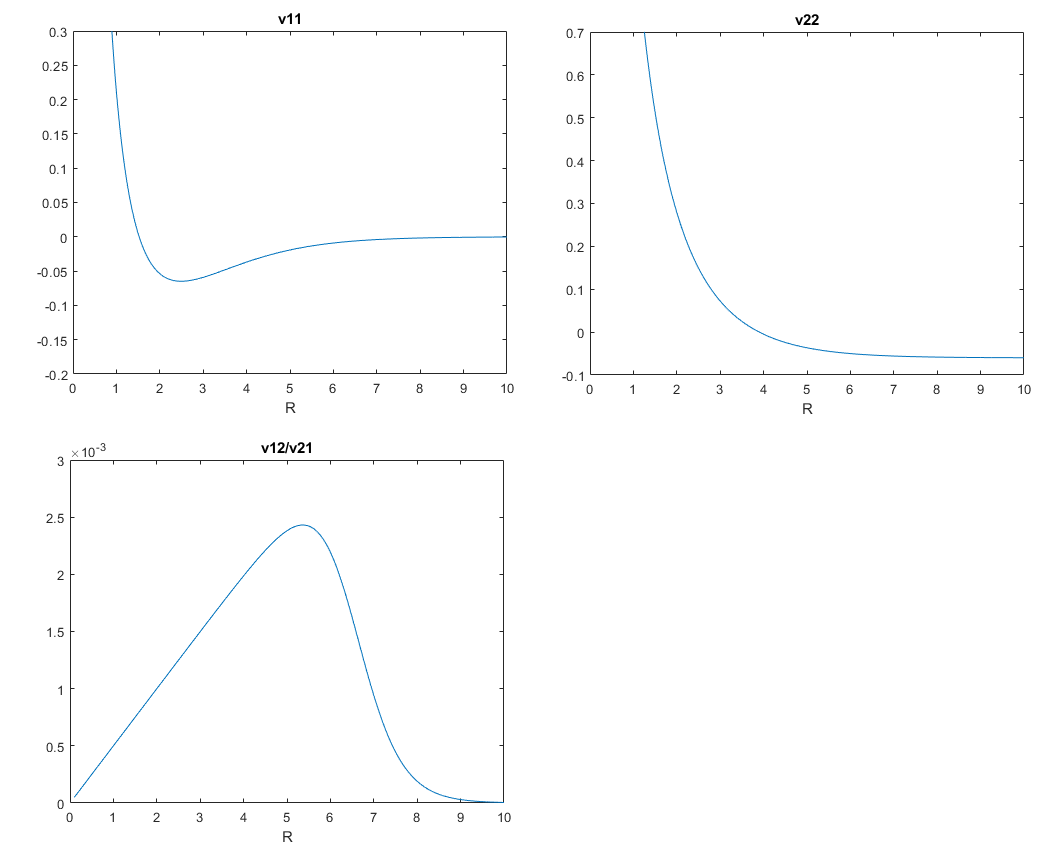
\includegraphics[width=14cm]{./figures/A2HW21.png}
\end{figure}

The radial TDSE with no couplint is
\begin{equation}
-\frac{1}{2\mu} \dv[2]{R} F_i(r) + V_{i,i} F_i(r) = E F_i(r) \qquad (i = 1, 2)
\end{equation}

Using finite difference method with equally space grid, the bound state energies for $V_{11}$ are
\begin{equation}
\ali{
&E_1 = -0.0607  & \qquad & E_2 = -0.0530 & \qquad & E_3 = -0.0457\\
&E_4 = -0.0388 && E_5 = -0.0325 && E_6 = -0.0267\\
&E_7 = -0.0214 && E_8 = -0.0167 && E_9 = -0.0124\\
&E_{10} = -0.00878 && E_{11} = -0.00571 && E_{12} = -0.00325\\
&E_{13} = -0.00144 && E_{14} = -0.000334
}\end{equation}
there is no bound states for $V_{22}$ because it's a monotonically decreasing function. So there is no bound states of total $\vec F$.



